% Document setup
%-----------------------------------------------------------------------------%
\documentclass[11pt]{article}
\usepackage[a4paper, margin=1.5cm]{geometry}
\raggedright
\usepackage[parfill]{parskip}
\usepackage{graphicx}
%-----------------------------------------------------------------------------%
% Import packages
%-----------------------------------------------------------------------------%
\usepackage{amsmath}
%-----------------------------------------------------------------------------%

% The document itself
%-----------------------------------------------------------------------------%
\begin{document}
%-----------------------------------------------------------------------------%
\section{DC Motor Circuit}
As an electrical schematic a DC motor can be represented as:
\begin{figure}[h]
  \centering
  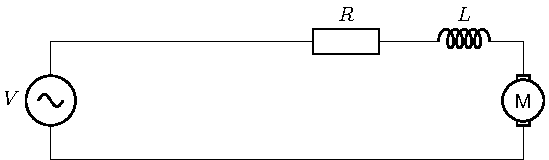
\includegraphics{motor_schematic/motor_schematic.pdf}
  \caption{Electrical diagram of DC motor.}
\end{figure}

By introducing an armature constant of the motor $K_t$, the torque the motor produces, $T$, is related to the armature current of the motor by:
\begin{equation}
  T = K_t i
\end{equation}

Similarly the motor back emf, $e$, is related to the rotational speed, $\dot{\theta}$ using the motor constant $K_e$ by:
\begin{equation}
  e = K_e \dot{\theta}
\end{equation}

From Kirchhoff's law the sum of potential differences in a closed loop must be zero. This leads to:
\begin{equation}
  iR + \frac{di}{dt}L = V - k_e\dot{\theta}
\end{equation}

\section{Inertia}
The inertia of the motor armature must also be considered.
From Newton's second law:
\begin{equation}
  J\ddot{\theta} + B\dot{\theta} = T
\end{equation}

Where $J$ is the motor inertial constant, and $B$ the motor damping constant.

\section{State-space Equations}
The following equations:
\begin{subequations}
  \begin{align}
    iR + \frac{di}{dt}L &= V - k_e\dot{\theta} \\
    J\ddot{\theta} + B\dot{\theta} &= T
  \end{align}
\end{subequations}

can be written in state-space form.
Selecting $\dot{\theta}$, $\ddot{\theta}$ and $i$ as the state variables:
\begin{equation}
  \dot{\theta} = \dot{\theta}
\end{equation}

For the inertia:
\begin{subequations}
  \begin{align}
    J\ddot{\theta} + B\dot{\theta} &= T \\
    \ddot{\theta} + \frac{B}{J}\dot{\theta} &= \frac{T}{J} \\
    \ddot{\theta} &= \frac{T}{J} - \frac{B}{J}\dot{\theta} \\
    \ddot{\theta} &= i\frac{K_t}{J} - \frac{B}{J}\dot{\theta} \\
  \end{align}
\end{subequations}

For Kirchhoff's law:
\begin{subequations}
  \begin{align}
    iR + \frac{di}{dt}L &= V - k_e\dot{\theta} \\
    i\frac{R}{L} + \frac{di}{dt} &= \frac{V}{L} - \frac{k_e}{L}\dot{\theta} \\
    \frac{di}{dt} &= \frac{V}{L} - \frac{k_e}{L}\dot{\theta} - i\frac{R}{L}\\
  \end{align}
\end{subequations}

Using $V$ as the input, and the motor position as the output:
\begin{subequations}
  \begin{align}
    \begin{bmatrix}
      \dot{\theta} \\
      \ddot{\theta} \\
      \frac{di}{dt}
    \end{bmatrix}
    &=
    \begin{bmatrix}
      0 & 1 & 0 \\
      0 & -\frac{B}{J} & \frac{K_t}{J} \\
      0 & -\frac{k_e}{L} & -\frac{R}{L}
    \end{bmatrix}
    \begin{bmatrix}
      \theta \\
      \dot{\theta} \\
      i
    \end{bmatrix}
    +
    \begin{bmatrix}
      0 \\
      0 \\
      \frac{1}{L}
    \end{bmatrix}
    V \\
    y &=
    \begin{bmatrix}
      1 & 0 & 0
    \end{bmatrix}
    \begin{bmatrix}
      \theta \\
      \dot{\theta} \\
      i
    \end{bmatrix}
  \end{align}
\end{subequations}
%-----------------------------------------------------------------------------%
\end{document}
%-----------------------------------------------------------------------------%
